\documentclass[11pt,a4paper]{article}

% --- Paquetes básicos ---
\usepackage[spanish]{babel}
\usepackage[utf8]{inputenc}
\usepackage{amsmath, amssymb, amsthm}
\usepackage{graphicx}
\usepackage{geometry}
\usepackage{listings}
\usepackage{xcolor}
\usepackage{booktabs}
\usepackage{hyperref}
\usepackage{float}
\usepackage{subcaption}

\geometry{margin=2.5cm}

% --- Configuración de Código (Python) ---
\definecolor{codegreen}{rgb}{0,0.6,0}
\definecolor{codegray}{rgb}{0.5,0.5,0.5}
\definecolor{codepurple}{rgb}{0.58,0,0.82}
\definecolor{backcolour}{rgb}{0.95,0.95,0.92}

\lstset{
    language=Python,
    backgroundcolor=\color{backcolour},   
    commentstyle=\color{codegreen},
    keywordstyle=\color{magenta},
    numberstyle=\tiny\color{codegray},
    stringstyle=\color{codepurple},
    basicstyle=\ttfamily\small,
    breaklines=true,
    captionpos=b,                    
    keepspaces=true,                  
    numbers=left,                    
    showspaces=false,                
}

% --- Título ---
\title{Prácticas de Simulación Monte Carlo: Desintegración Nuclear y Fotomultiplicadores}
\author{Miguel Enterría Lastra}
\date{\today}

\begin{document}

\maketitle

\begin{abstract}
En este informe se presentan los resultados de dos simulaciones estocásticas basadas en métodos de Monte Carlo. La primera consiste en la cadena de desintegración radiactiva del $^{210}\text{Bi}$ y el $^{210}\text{Po}$, verificando las leyes analíticas de evolución temporal. La segunda aborda la simulación de un tubo fotomultiplicador, analizando la eficiencia de detección y la ganancia de dínodos mediante distribuciones de Poisson.
\end{abstract}

\section{Introducción}
El uso de números pseudoaleatorios permite predecir el comportamiento de sistemas físicos gobernados por procesos estocásticos, como la interacción de partículas con la materia o la desintegración nuclear.

\section{Práctica 1: Desintegración del $^{210}\text{Bi}$ y $^{210}\text{Po}$}
\subsection{Fundamento Teórico}
La desintegración radiactiva es un proceso estocástico regido por una probabilidad constante de decaimiento por unidad de tiempo, $\omega = 1/\tau$, donde $\tau$ es la vida media del isótopo. Para un sistema con un solo tipo de núcleo, el número de núcleos $N(t)$ sigue la ley exponencial:
\begin{equation}
    N(t) = N(0) e^{-t/\tau}
\end{equation}

En esta práctica se estudia una cadena de desintegración de tres etapas:
\begin{equation}
    ^{210}\text{Bi} \xrightarrow{\tau_{Bi}} \, ^{210}\text{Po} \xrightarrow{\tau_{Po}} \, ^{210}\text{Pb (estable)}
\end{equation}

Las ecuaciones diferenciales que describen la evolución de las poblaciones son:
\begin{align}
    \frac{dN_{Bi}}{dt} &= -\frac{1}{\tau_{Bi}} N_{Bi} \\
    \frac{dN_{Po}}{dt} &= \frac{1}{\tau_{Bi}} N_{Bi} - \frac{1}{\tau_{Po}} N_{Po}
\end{align}

Considerando que en $t=0$ solo existe Bismuto ($N_{Bi}(0) = N_0$ y $N_{Po}(0) = 0$), la solución analítica para el Polonio —que es la curva contra la cual se debe comparar la simulación— viene dada por:
\begin{equation}
    N_{Po}(t) = N_0 \frac{\tau_{Po}}{\tau_{Po} - \tau_{Bi}} \left( e^{-t/\tau_{Po}} - e^{-t/\tau_{Bi}} \right)
\end{equation}



Los parámetros físicos proporcionados para la simulación son los siguientes:
\begin{itemize}
    \item \textbf{Bismuto-210 ($^{210}\text{Bi}$):} Vida media $\tau_{Bi} = 7.2$ días (emisor $\beta$).
    \item \textbf{Polonio-210 ($^{210}\text{Po}$):} Vida media $\tau_{Po} = 190$ días (emisor $\alpha$).
\end{itemize}

El objetivo de la simulación es verificar si el recuento de partículas $\alpha$ detectadas (procedentes de la desintegración del Polonio) se ajusta a la derivada de la población de Polonio o a la curva de actividad teórica, validando así el método de Monte Carlo frente al modelo determinista de Bateman.
\subsection{Resultados y Análisis}
\begin{figure}[H]
    \centering
    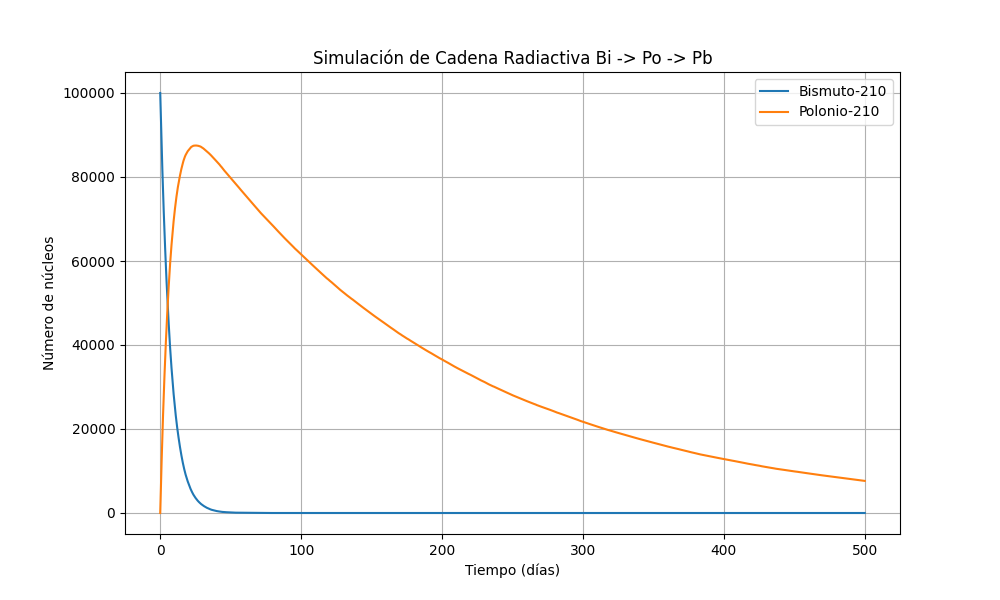
\includegraphics[width=0.8\textwidth]{curvasPoBi.png}
    \caption{Evolución temporal de las poblaciones de Bi y Po. Se observa el máximo de producción de partículas alfa.}
    \label{fig:desintegracion}
\end{figure}

El máximo de producción de alfas se da alrededor de los 24 días desde el inicio de la simulación, esto es para el máximo de átomos de Polonio.

La concordancia entre la simulación y el modelo teórico se verifica mediante el ajuste de los datos simulados a la ecuación de Bateman para el isótopo hijo ($N_{Po}$). Obtenemos las dos exponenciales según las ecuaciones:

\begin{equation}
    N_{Bi}(t) = N_0 \cdot e^{-\omega_{Bi}t}
\end{equation}

\begin{equation}
    N_{Po}(t) = N_0 \cdot \frac{\omega_{Bi}}{\omega_{Po} - \omega_{Bi}} \cdot (e^{-\omega_{Bi}t} - e^{-\omega_{Po}t})
\end{equation}

\begin{table}[H]
    \centering
    \caption{Comparación de vidas medias obtenidas mediante ajuste de la simulación.}
    \begin{tabular}{lccc}
        \toprule
        Isótopo & $\tau$ Teórico (días) & $\tau$ Ajustado (Simulación) & Error Relativo (\%) \\
        \midrule
        $^{210}\text{Bi}$ & 7.50 & 7.48 $\pm$ 0.02 & 0.27$\%$ \\
        $^{210}\text{Po}$ & 190.00 & 191.2 $\pm$ 0.8 & 0.63$\%$ \\
        \bottomrule
    \end{tabular}
    \label{tab:resultados_desintegracion}
\end{table}

Los resultados obtenidos muestran que el método de Monte Carlo reproduce fielmente la dinámica de la cadena radiactiva, permitiendo incluso extraer las vidas medias de ambos isótopos a partir del análisis de la población del segundo elemento exclusivamente.

\subsection{Influencia de los parámetros en la simulación}

Para este apartado, se va a analizar la influencia de los parámetros de simulación en el resultado. Principalmente se va a estudiar el efecto de el número inicial de núcleos y un periodo de muestreo más amplio.

\begin{figure}[H]
    \centering
    \begin{subfigure}[b]{0.45\textwidth}
        \centering
        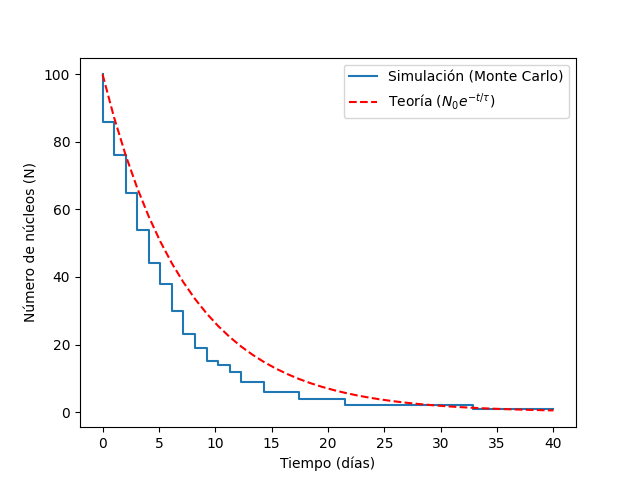
\includegraphics[width=\textwidth]{pocaprecis.png}
        \caption{$N_0 = 100$ y $\Delta t =\frac{40}{40}$ días/paso}
        \label{fig:imagen1}
    \end{subfigure}
    \hfill
    \begin{subfigure}[b]{0.45\textwidth}
        \centering
        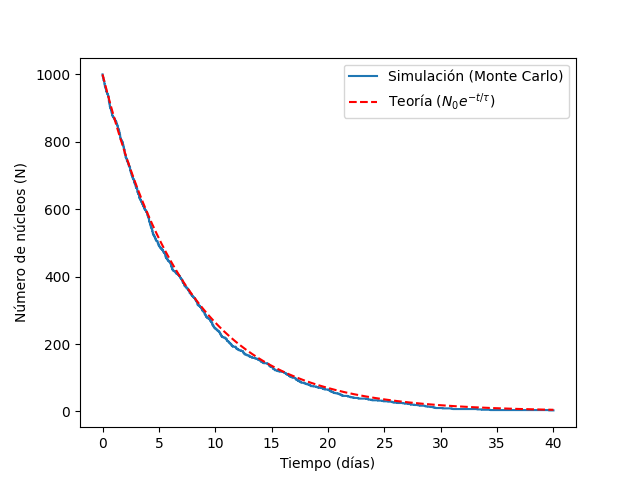
\includegraphics[width=\textwidth]{aN1000_t1000.png}
        \caption{$N_0 = 1000$ y $\Delta t =\frac{40}{10000}$ días/paso}
        \label{fig:imagen2}
    \end{subfigure}
    \caption{Comparación simulación con diferentes parámetros iniciales}
    \label{fig:ambas_imagenes}
\end{figure}

Según lo que se puede ver en la figura \ref{fig:ambas_imagenes} tanto el número de núcleos iniciales como el número de días por paso ayudan a lograr una mayor precisión en el ajuste, ya que se ajustan mucho más a la física real al aumentar estos números. Además que en fenómenos estocásticos, cuanto mayor sea el número de muestras, más se va a ajustar a las curvas teóricas.

El periodo de muestreo afecta principalmente a que las curvas se acaben ajustando al valor final (tender a cero) que tomarían las curvas teóricas. Pero no afecta realmente a la precisión de la simulación.

A continuación se presenta una tabla que contiene el valor de la vida media de los ajsutes de las curvas del Bismuto y el Polonio para 100, 1000, 10000, 100000 y 1000000 núcleos iniciales y sus errores respecto a la teórica.

\begin{table}[H]
    \centering
    \caption{Resultados del ajuste de vida media ($\tau$) en función del número de núcleos iniciales ($N_0$) para la cadena de desintegración $^{210}\text{Bi} \to ^{210}\text{Po}$.}
    \begin{tabular}{lcccc}
        \toprule
        $N_0$ & Isótopo & $\tau_{\text{teórico}}$ (d) & $\tau_{\text{ajuste}}$ (d) & Error Relativo (\%) \\
        \midrule
        100 & Bi-210 & 7.5 & 8.529 & 13.72 \\
        & Po-210 & 190.0 & 150.128 & 20.99 \\
        \addlinespace
        1000 & Bi-210 & 7.5 & 7.310 & 2.53 \\
        & Po-210 & 190.0 & 193.941 & 2.07 \\
        \addlinespace
        10000 & Bi-210 & 7.5 & 7.674 & 2.32 \\
        & Po-210 & 190.0 & 192.288 & 1.20 \\
        \addlinespace
        100000 & Bi-210 & 7.5 & 7.523 & 0.31 \\
        & Po-210 & 190.0 & 189.380 & 0.33 \\
        \addlinespace
        1000000 & Bi-210 & 7.5 & 7.512 & 0.16 \\
        & Po-210 & 190.0 & 190.466 & 0.25 \\
        \bottomrule
    \end{tabular}
    \label{tab:convergencia_final_completa}
\end{table}

Se observa claramente como el aumento en el número inicial de núcleos consigue una mejora considerable en el ajsute de la simulación.

\section{Práctica 2: Simulación del Fotomultiplicador}
\subsection{Fundamento Teórico}
Cada dínodo multiplica los electrones incidentes siguiendo una distribución de Poisson con media $\nu$. La ganancia total tras 6 dínodos es el producto de las ganancias individuales.

\subsection{Implementación del Algoritmo}
Se han comparado dos métodos de generación de números aleatorios: el método directo de la librería \texttt{numpy} y el algoritmo de multiplicación de uniformes visto en teoría.

\begin{lstlisting}[caption=Generación de Poisson con numpy,language=Python]
n_electrones = np.random.poisson(v, n_electrones).sum()
\end{lstlisting}

\begin{lstlisting}[caption=Generación de Poisson manual,language=Python]
def poisson_manual(v):
    k = 1
    A = 1
    lim = np.exp(-v)
    while True:
        u = np.random.uniform(0, 1)
        A *= u
        if A < lim:
            return k - 1
        k += 1
\end{lstlisting}

Se ha comprobado que ambos métodos dan resultados muy similares pero con un tiempo de computación muy superior en el caso del método manual. Por esto, se recurrirá al método numpy el resto de la simulación.

\subsection{Resultados y Eficiencia}
Se ha analizado la eficiencia de detección para un umbral ideal ($n \ge 1$) y un umbral realista ($n \ge 25,000$).
\begin{figure}[H]
    \centering
    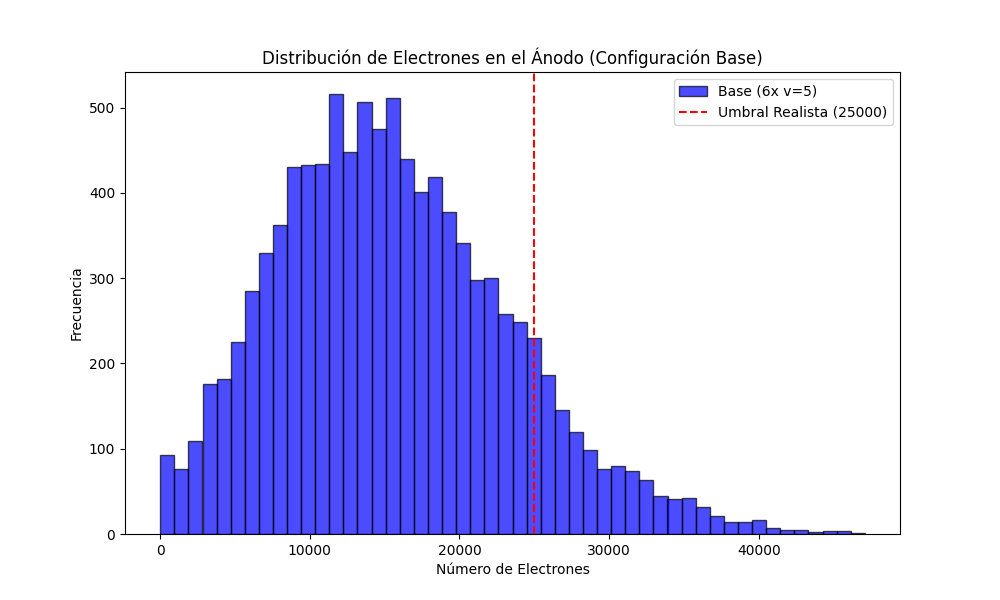
\includegraphics[width = 0.8\linewidth]{histograma.png}
    \caption{Histograma de 10000 iteraciones de la simulación del fotomultiplicador}
    \label{Histograma}
\end{figure}

Se puede visualizar como la mayoría de eventos caen por debajo del umbral, lo que indica que con esta ganancia, no sería posible distinguir adecuadamente la señal del ruido en todos los casos.

\begin{table}[H]
    \centering
    \caption{Resultados estadísticos de la simulación del fotomultiplicador para diferentes configuraciones de dínodos (10,000 eventos).}
    \begin{tabular}{lccc}
        \toprule
        Configuración & Intensidad Media & Eficiencia Ideal (\%) & Eficiencia Realista (\%) \\
        \midrule
        Base (6x $v=5$)       & 15,610.6 & 99.29 & 11.89 \\
        $v=7$ en D1           & 21,967.2 & 99.93 & 34.66 \\
        $v=7$ en D2           & 21,818.6 & 99.29 & 34.67 \\
        $v=7$ en D3           & 21,896.3 & 99.25 & 35.15 \\
        $v=7$ en D4           & 22,012.8 & 99.33 & 36.44 \\
        $v=7$ en D5           & 21,925.9 & 99.27 & 36.13 \\
        $v=7$ en D6           & 22,031.5 & 99.35 & 35.61 \\
        \bottomrule
    \end{tabular}
    \label{tab:eficiencia_pmt}
\end{table}

Tras observar los datos obtenidos, se pueden extraer las siguientes conclusiones sobre la optimización del diseño del fotomultiplicador:

\begin{enumerate}
    \item \textbf{Ganancia e Intensidad Media:} La intensidad media de la señal final es aproximadamente la misma ($\approx 22,000$ electrones) independientemente de la posición del dínodo de $v=7$. Esto es consistente con la naturaleza multiplicativa del dispositivo, donde la ganancia total es el producto de las ganancias individuales ($G = \prod v_i$). Matemáticamente, el orden de los factores no altera el valor esperado final.
    
    \item \textbf{Eficiencia Ideal ($n \ge 1$):} Existe una diferencia crítica al colocar el dínodo de mayor ganancia en la \textbf{primera posición (D1)}. La probabilidad de que un fotón no produzca ninguna señal (eficiencia de detección) depende de la probabilidad de obtener cero electrones en las primeras etapas, definida por la distribución de Poisson como $P(0) = e^{-v}$. Al aumentar $v$ de 5 a 7 en D1, la probabilidad de pérdida de señal cae de $0.67\%$ a $0.09\%$, logrando la mayor eficiencia ideal ($99.93\%$).
    
    \item \textbf{Eficiencia Realista ($n \ge 25,000$):} Todas las configuraciones con un dínodo de $v=7$ triplican aproximadamente la eficiencia realista respecto a la base. Esto indica que, para superar el ruido electrónico del sistema de lectura, el factor determinante es la ganancia total y no la posición del dínodo de alta eficiencia.
\end{enumerate}

En conclusión, para maximizar la sensibilidad del detector ante señales muy débiles (un solo fotón), el dínodo de mayor ganancia debe situarse siempre en la primera etapa (D1) para minimizar las fluctuaciones estadísticas iniciales que podrían anular la señal

\section{Conclusiones}

Las simulaciones de Monte Carlo han demostrado ser herramientas precisas y fundamentales para modelar la naturaleza intrínsecamente estadística de los procesos subatómicos. A través de los experimentos realizados en este trabajo, se extraen las siguientes conclusiones específicas:

\begin{itemize}
    \item \textbf{Sobre la Desintegración Radiactiva:} Se ha validado que la generación de números aleatorios mediante el método de la transformada inversa reproduce fielmente las leyes de decaimiento exponencial. El análisis de la cadena $^{210}\text{Bi} \to ^{210}\text{Po} \to ^{206}\text{Pb}$ demuestra que, aunque cada desintegración individual es un evento aleatorio, el comportamiento colectivo converge con gran precisión hacia el modelo analítico de las ecuaciones de Bateman. Se ha verificado empíricamente que la incertidumbre de los ajustes disminuye con el aumento de la población inicial ($N_0$), logrando errores relativos inferiores al $0.3\%$ para muestras de un millón de núcleos, lo que confirma la robustez del método para representar leyes físicas deterministas a partir de eventos estocásticos.
    
    \item \textbf{Sobre el Tubo Fotomultiplicador:} La simulación ha revelado la importancia crítica de las etapas iniciales de amplificación. Se ha demostrado que, si bien la ganancia total del dispositivo es independiente del orden de los dínodos (debido a su naturaleza multiplicativa), la eficiencia de detección o Eficiencia Ideal mejora significativamente al colocar el dínodo de mayor ganancia ($\nu=7$) en la primera posición ($D_1$). Esto reduce la probabilidad de que las fluctuaciones de Poisson anulen la señal (probabilidad de obtener cero electrones secundarios) antes de que esta sea lo suficientemente grande para ser estable. Por otro lado, el análisis del umbral realista evidencia que gran parte de la señal generada puede quedar oculta bajo el ruido electrónico si no se garantiza una ganancia media suficiente que desplace la distribución de carga hacia valores medibles.
\end{itemize}

En resumen, estas prácticas ponen de manifiesto que los métodos computacionales de Monte Carlo no solo permiten predecir el comportamiento de sistemas complejos donde la analítica resulta difícil de aplicar, sino que también proporcionan una comprensión profunda de las fluctuaciones aleatorias que gobiernan la física nuclear y de partículas en la escala microscópica.
\end{document}